% Options for packages loaded elsewhere
\PassOptionsToPackage{unicode}{hyperref}
\PassOptionsToPackage{hyphens}{url}
%
\documentclass[
]{article}
\usepackage{amsmath,amssymb}
\usepackage{lmodern}
\usepackage{iftex}

\usepackage{geometry}
\geometry{letterpaper, margin=1in}

\ifPDFTeX
  \usepackage[T1]{fontenc}
  \usepackage[utf8]{inputenc}
  \usepackage{textcomp} % provide euro and other symbols
\else % if luatex or xetex
  \usepackage{unicode-math}
  \defaultfontfeatures{Scale=MatchLowercase}
  \defaultfontfeatures[\rmfamily]{Ligatures=TeX,Scale=1}
\fi
% Use upquote if available, for straight quotes in verbatim environments
\IfFileExists{upquote.sty}{\usepackage{upquote}}{}
\IfFileExists{microtype.sty}{% use microtype if available
  \usepackage[]{microtype}
  \UseMicrotypeSet[protrusion]{basicmath} % disable protrusion for tt fonts
}{}
\makeatletter
\@ifundefined{KOMAClassName}{% if non-KOMA class
  \IfFileExists{parskip.sty}{%
    \usepackage{parskip}
  }{% else
    \setlength{\parindent}{0pt}
    \setlength{\parskip}{6pt plus 2pt minus 1pt}}
}{% if KOMA class
  \KOMAoptions{parskip=half}}
\makeatother
\usepackage{xcolor}
\IfFileExists{xurl.sty}{\usepackage{xurl}}{} % add URL line breaks if available
\IfFileExists{bookmark.sty}{\usepackage{bookmark}}{\usepackage{hyperref}}
\hypersetup{
  hidelinks,
  pdfcreator={LaTeX via pandoc}}
\urlstyle{same} % disable monospaced font for URLs
\usepackage{graphicx}
\makeatletter
\def\maxwidth{\ifdim\Gin@nat@width>\linewidth\linewidth\else\Gin@nat@width\fi}
\def\maxheight{\ifdim\Gin@nat@height>\textheight\textheight\else\Gin@nat@height\fi}
\makeatother
% Scale images if necessary, so that they will not overflow the page
% margins by default, and it is still possible to overwrite the defaults
% using explicit options in \includegraphics[width, height, ...]{}
\setkeys{Gin}{width=\maxwidth,height=\maxheight,keepaspectratio}
% Set default figure placement to htbp
\makeatletter
\def\fps@figure{htbp}
\makeatother
\setlength{\emergencystretch}{3em} % prevent overfull lines
\providecommand{\tightlist}{%
  \setlength{\itemsep}{0pt}\setlength{\parskip}{0pt}}
\setcounter{secnumdepth}{-\maxdimen} % remove section numbering
\ifLuaTeX
  \usepackage{selnolig}  % disable illegal ligatures
\fi

\author{}
\date{}

\begin{document}

\hypertarget{proyecto-1---diseuxf1o-y-anuxe1lisis-de-algoritmos}{%
\section{Proyecto 1 - Diseño y análisis de
algoritmos}\label{proyecto-1---diseuxf1o-y-anuxe1lisis-de-algoritmos}}

\textbf{Realizado por:}

\begin{itemize}
\tightlist
\item
  Juan David Guevara Arévalo - 202116875
\item
  Jose David Martínez Oliveros - 202116677
\end{itemize}

\hypertarget{algoritmo-de-soluciuxf3n}{%
\subsection{1. Algoritmo de solución}\label{algoritmo-de-soluciuxf3n}}

Para solucionar el problema, se decidió abordarlo en 3 etapas:

\begin{enumerate}
\def\labelenumi{\arabic{enumi}.}
\tightlist
\item
  Determinar un algoritmo para ordenar las torres (sin pensar en hacerlo
  de la mejor forma)
\item
  Mejorar el algoritmo para obtener la menor cantidad de pasos.
\item
  Optimizar el algoritmo para reducir el tiempo de ejecución.
\end{enumerate}

\hypertarget{determinar-un-algoritmo-para-solucionar-el-problema}{%
\subsubsection{1.1. Determinar un algoritmo para solucionar el
problema}\label{determinar-un-algoritmo-para-solucionar-el-problema}}

Para llegar a un algoritmo, se planteo la situación más pequeña posible
(donde tan solo hay 2 torres) y planteamos una ecuación de recurrencia
que solucionaría dicha situación. La ecuación encontrada es la
siguiente:

\begin{verbatim}
dp[i] = dp[i] + ceil((dp[i + 1] - dp[i]) / 2) if dp[i + 1] > dp[i]
dp[i + 1] = dp[i + 1] - ceil((dp[i + 1] - dp[i]) / 2) if dp[i + 1] > dp[i]
\end{verbatim}

La anterior ecuación, aumenta la torre \(i\) la cantidad de pasos
requeridos, a la vez que decrementa la torre \(i+1\).

Sin embargo, para completar el algoritmo, es necesario iterar
(\emph{Mover \(i\)}) correctamente para conseguir un método funcional.
Para ello, identificamos el caso en el que hay 3 torres, y se está
revisando la torre del medio. Una vez aplicada la ecuación, es necesario
revisar que la torre del medio siga siendo más alta o igual que la
anterior, si no lo es, se decrementa \(i\), de lo contrario se
incrementa.

Con dicha estrategia, el algoritmo ya ordena las torres correctamente.

\hypertarget{obtener-la-menor-cantidad-de-pasos}{%
\subsubsection{1.2. Obtener la menor cantidad de
pasos}\label{obtener-la-menor-cantidad-de-pasos}}

Dado que a una torre es posible ponerle fichas de cualquier torre
adyacente, es necesario actualizar el algoritmo para que tome las fichas
del mejor lado y no solo de la izquierda. Para ello, es necesario
calcular la diferencia de altitud entre las torre \(i\) e \(i + 1\), y
ver si podemos obtener dicha cantidad de la torre izquierda sin hacerla
más pequeña que la altura objetivo. Esto asegura que, de ser posible,
nivelaremos la torre actual asegurando que siga siendo menor o igual a
la de la izquierda. La ecuación de recurrencia final sería la siguiente:

\begin{verbatim}
diff = dp[i + 1] - dp[i] # Por simplicidad

dp[i] = dp[i] if i == n - 1 or diff <= 0
dp[i] = dp[i] + ceil(diff / 2) if i == 0 or floor((dp[i-1] - dp[i]) / 2) < diff
dp[i] = dp[i] + min(floor((dp[i-1] - dp[i]) / 2), diff)
\end{verbatim}

\emph{Por simplicidad se omitió la actualización de \(dp[i - 1]\) y
\(dp[i + 1]\) respectivamente.}

Implementando la anterior ecuación, las torres no solo terminarán en el
orden correcto, sino que el proceso se realizará en la menor cantidad de
pasos posibles. \emph{Solución final del proyecto.}

\hypertarget{optimizaciuxf3n}{%
\subsubsection{1.3. Optimización}\label{optimizaciuxf3n}}

\emph{A partir de aquí la implementación en código se aleja un poco de
la ecuación de recurrencia definida, sin embargo, sigue la misma
estrategia de tomar de la izquierda si es posible, de lo contrario de la
derecha.}

Para optimizar el algoritmo fue necesario reducir considerablemente la
cantidad de iteraciones realizadas. Para ello se enfrentaron 2 problemas:

\begin{itemize}
\tightlist
\item
  Agilizar la cantidad de iteraciones requeridas para ordenar casos
  sencillos.
\item
  Identificar desde que punto las torres tienen el mismo tamaño
\end{itemize}

El primer punto fue sencillo, ya que es fácil saber como deben quedar
las torres si hay \(N\) torres seguidas del mismo tamaño \(n\) y luego
aparece una torre de altura \(n + k\).

\begin{verbatim}
      N
 |----------|                
|            #|            |             |
|            #|     ->     |##           |
|#############|            |#############|
Donde la altura n es 1, y la diferencia k es 2.
\end{verbatim}

Tras varias pruebas, la formula identificada para calcular la cantidad
de pasos necesarios para ordenar el caso descrito fue la siguiente:

\(B = \frac{k}{N}\) \emph{~~Tomando únicamente la parte entera}

\(r = k - B\cdot N\) \emph{~~Es el residuo de dividir \(k\) entre \(N\)}

\(R = N - r\) \emph{~~La cantidad de pasos que hay que restar}

\(steps = \frac{1}{2}N(B + 1)(N+1) - \frac{1}{2}R(R+1)\)

Con la disponibilidad de esta formula, lo único que resta es hacer un
traqueo correcto de la posición desde la que hay una región aplanada
para identificar \(N\) de forma adecuada.

Para ello, se creó una variable auxiliar con el objetivo de guardar la
posición desde la cual hay torres del mismo tamaño seguidas. La forma de
aumentar el valor de dicha variable es sencilla, pues si en el recorrido
actual de las torres la siguiente es más baja, se aumenta el valor de
dicha variable, de lo contrario no se modifica.

Cabe resaltar que una vez se actualizan las torres, es necesario
re-calcular el valor de la variable, lo cuál es sencillo en el caso
\(N > k\), de lo contrario, simplemente \(i\) se actualiza con valor 0.

\emph{Para mejorar aún más la complejidad temporal en lugar de utilizar
una variable, se puede utilizar una cola en la que se van guardando las
posiciones, pero se empieza a sacrificar memoria y la diferencia no es
tan significativa.}

\hypertarget{anuxe1lisis-de-complejidades-espacial-y-temporal}{%
\subsection{2. Análisis de complejidades espacial y
temporal}\label{anuxe1lisis-de-complejidades-espacial-y-temporal}}

\hypertarget{complejidad-temporal}{%
\subsubsection{2.1. Complejidad temporal}\label{complejidad-temporal}}

\textbf{Mejor caso}

Tras las optimizaciones, el algoritmo tiene dos casos donde la
complejidad será \(O(n)\).

\begin{enumerate}
\def\labelenumi{\arabic{enumi}.}
\tightlist
\item
  El primero, y obvio, es cuando todas las torres están ordenadas y la
  complejidad exacta es \(\ T(n) = n\) ya que no se realiza ninguna
  operación.
\item
  El segundo, es cuando hay torres que están precedidas por una menos
  alta, pero tienen una región aplanada de superficie mayor o igual a la
  diferencia de altitud de dicha torre. Esto se debe a que podemos
  organizar fácilmente utilizando la formula presentada con
  anterioridad, sin reiniciar la variable \(i\) a \(0\), por lo que la
  complejidad exacta es \(\ T(n) = 2n\) por lo que la complejidad
  seguirá siendo \(O(n)\)
\end{enumerate}

\textbf{Caso Promedio}

Estimar la complejidad promedio puede ser una tarea difícil, sin
embargo, por la naturaleza del problema, donde la suma de las alturas de
las torres es menor a 10000, y la cantidad máxima de las torres también
es 10000, la mayoría de casos tendrán una buena cantidad de regiones
aplanadas. Por lo que el código, si bien no es \(\ T(n) = n\), es
\(\ T(n) = k\cdot n\) donde \(k\) es lo suficientemente pequeño para
considerar que sigue teniendo una complejidad \(O(n)\)

\emph{\textbf{Ver \protect\hyperlink{anexo-1}{Anexo 1}}; una gráfica del
tiempo en milésimas de segundo que le toma al algoritmo solucionar para
\(N\) torres, donde se cumplen las restricciones de los datos de
entrada.}

Es posible evidenciar, que si bien la gráfica no tiene una tendencia
clara, los picos tienen un crecimiento lineal (cada vez los picos son
mayores), esto se debe a que a medida que aumenta la cantidad de datos,
existen algunos puntos de inflexión que permiten utilizar una menor
cantidad de veces la estrategia de utilizar las zonas llanas, pero
claramente, cuanto más crezca la cantidad de torres, si se mantiene la
restricción de que los elementos no pueden sumar más de 10000, la
complejidad del algoritmo se estabilizará en \(\ T(n) = n\).

\textbf{Peor caso}

Para estimar la complejidad temporal en el peor de los casos, será
necesario ignorar las restricciones que tienen los datos. Y para ello,
se analizaron 2 escenarios y se estimó una complejidad temporal
\(O(n^2)\).

\textbf{1. Torres entre 0 y 10000 sin la restricción de la suma:} En
este caso, se utilizó un script de Python para producir entradas
completamente aleatorias, lo que hará que el algoritmo tenga que
reiniciar o decrementar una amplia cantidad de veces el iterador \(i\).
\textbf{\emph{Ver \protect\hyperlink{anexo-2}{Anexo 2}}} Una gráfica
donde se evidencia el resultado. \emph{Nótese que aún así, el algoritmo
maneja un excelente tiempo de ejecución.}

\textbf{2. Torres con altitud cuadrática:} Para este caso, con el
objetivo de poner en las peores circunstancias al algoritmo (ya que en
esta circunstancias la gran mayoría de las veces el algoritmo
retrocederá hasta \(i=0\) en cada torre) se creó un conjunto de datos en
el que la altura de cada torre, es la posición de la misma elevada al
cuadrado, está vez, es mucho más sencillo notar el crecimiento
cuadrático del tiempo. \textbf{\emph{Ver
\protect\hyperlink{anexo-3}{Anexo 3}}}

Tras estos análisis, se puede concluir que la complejidad temporal del
algoritmo es \(\ O(n)\) para la mayoría de casos dadas las
precondiciones definidas, sin embargo, sí se tienen en cuenta casos más
generales que no cumplan las precondiciones, la complejidad temporal
sería \(O(n^2)\).

\hypertarget{complejidad-espacial}{%
\subsubsection{2.2. Complejidad espacial}\label{complejidad-espacial}}

La complejidad espacial del algoritmo es \(O(1)\), pues para la
ejecución del mismo, no se maneja ningún arreglo auxiliar. Todas las
operaciones se realizan sobre el arreglo de entrada.

\hypertarget{escenarios}{%
\subsection{3. Escenarios}\label{escenarios}}

\hypertarget{en-un-movimiento-se-puede-mover-muxe1s-de-una-ficha}{%
\subsubsection{3.1. En un movimiento se puede mover más de una
ficha}\label{en-un-movimiento-se-puede-mover-muxe1s-de-una-ficha}}

Para este escenario, dada la implementación llevada a cabo en el código,
el único reto adicional que aparece, es actualizar la formula presentada
para calcular correctamente la cantidad de pasos. Por lo demás, se
debería actualizar el incremento de los pasos para que sea de uno en uno
en lugar de ser incrementados en función de la diferencia de alturas.

\hypertarget{se-pueden-mover-fichas-entre-torres-no-necesariamente-contiguas-pero-si-dentro-de-un-radio-de-r-torres.}{%
\subsubsection{\texorpdfstring{3.2. Se pueden mover fichas entre torres
no necesariamente contiguas, pero si dentro de un radio de \(r\)
torres.}{3.2. Se pueden mover fichas entre torres no necesariamente contiguas, pero si dentro de un radio de r torres.}}\label{se-pueden-mover-fichas-entre-torres-no-necesariamente-contiguas-pero-si-dentro-de-un-radio-de-r-torres.}}

Este escenario si comprende nuevos retos. En primer lugar, habría que
actualizar la formula casi por completo para que sea considerado el
radio \(r\), además, para las demás situaciones, habría que considerar
tener una nueva lista o cola auxiliar para identificar la mejor torre en
el radio a la cual pasar cada ficha.

Esto podría aumentar la complejidad espacial a \(O(n)\) (En el caso en
el que \(r > \frac{n}{2}\)). Además, la complejidad temporal podría
aumentar de \(O(n^2)\) en el peor caso a \(O(n^3)\).

\hypertarget{anexos}{%
\subsection{4. Anexos}\label{anexos}}

\hypertarget{anexo-1}{%
\subsubsection{4.1. Anexo 1}\label{anexo-1}}

\begin{center}
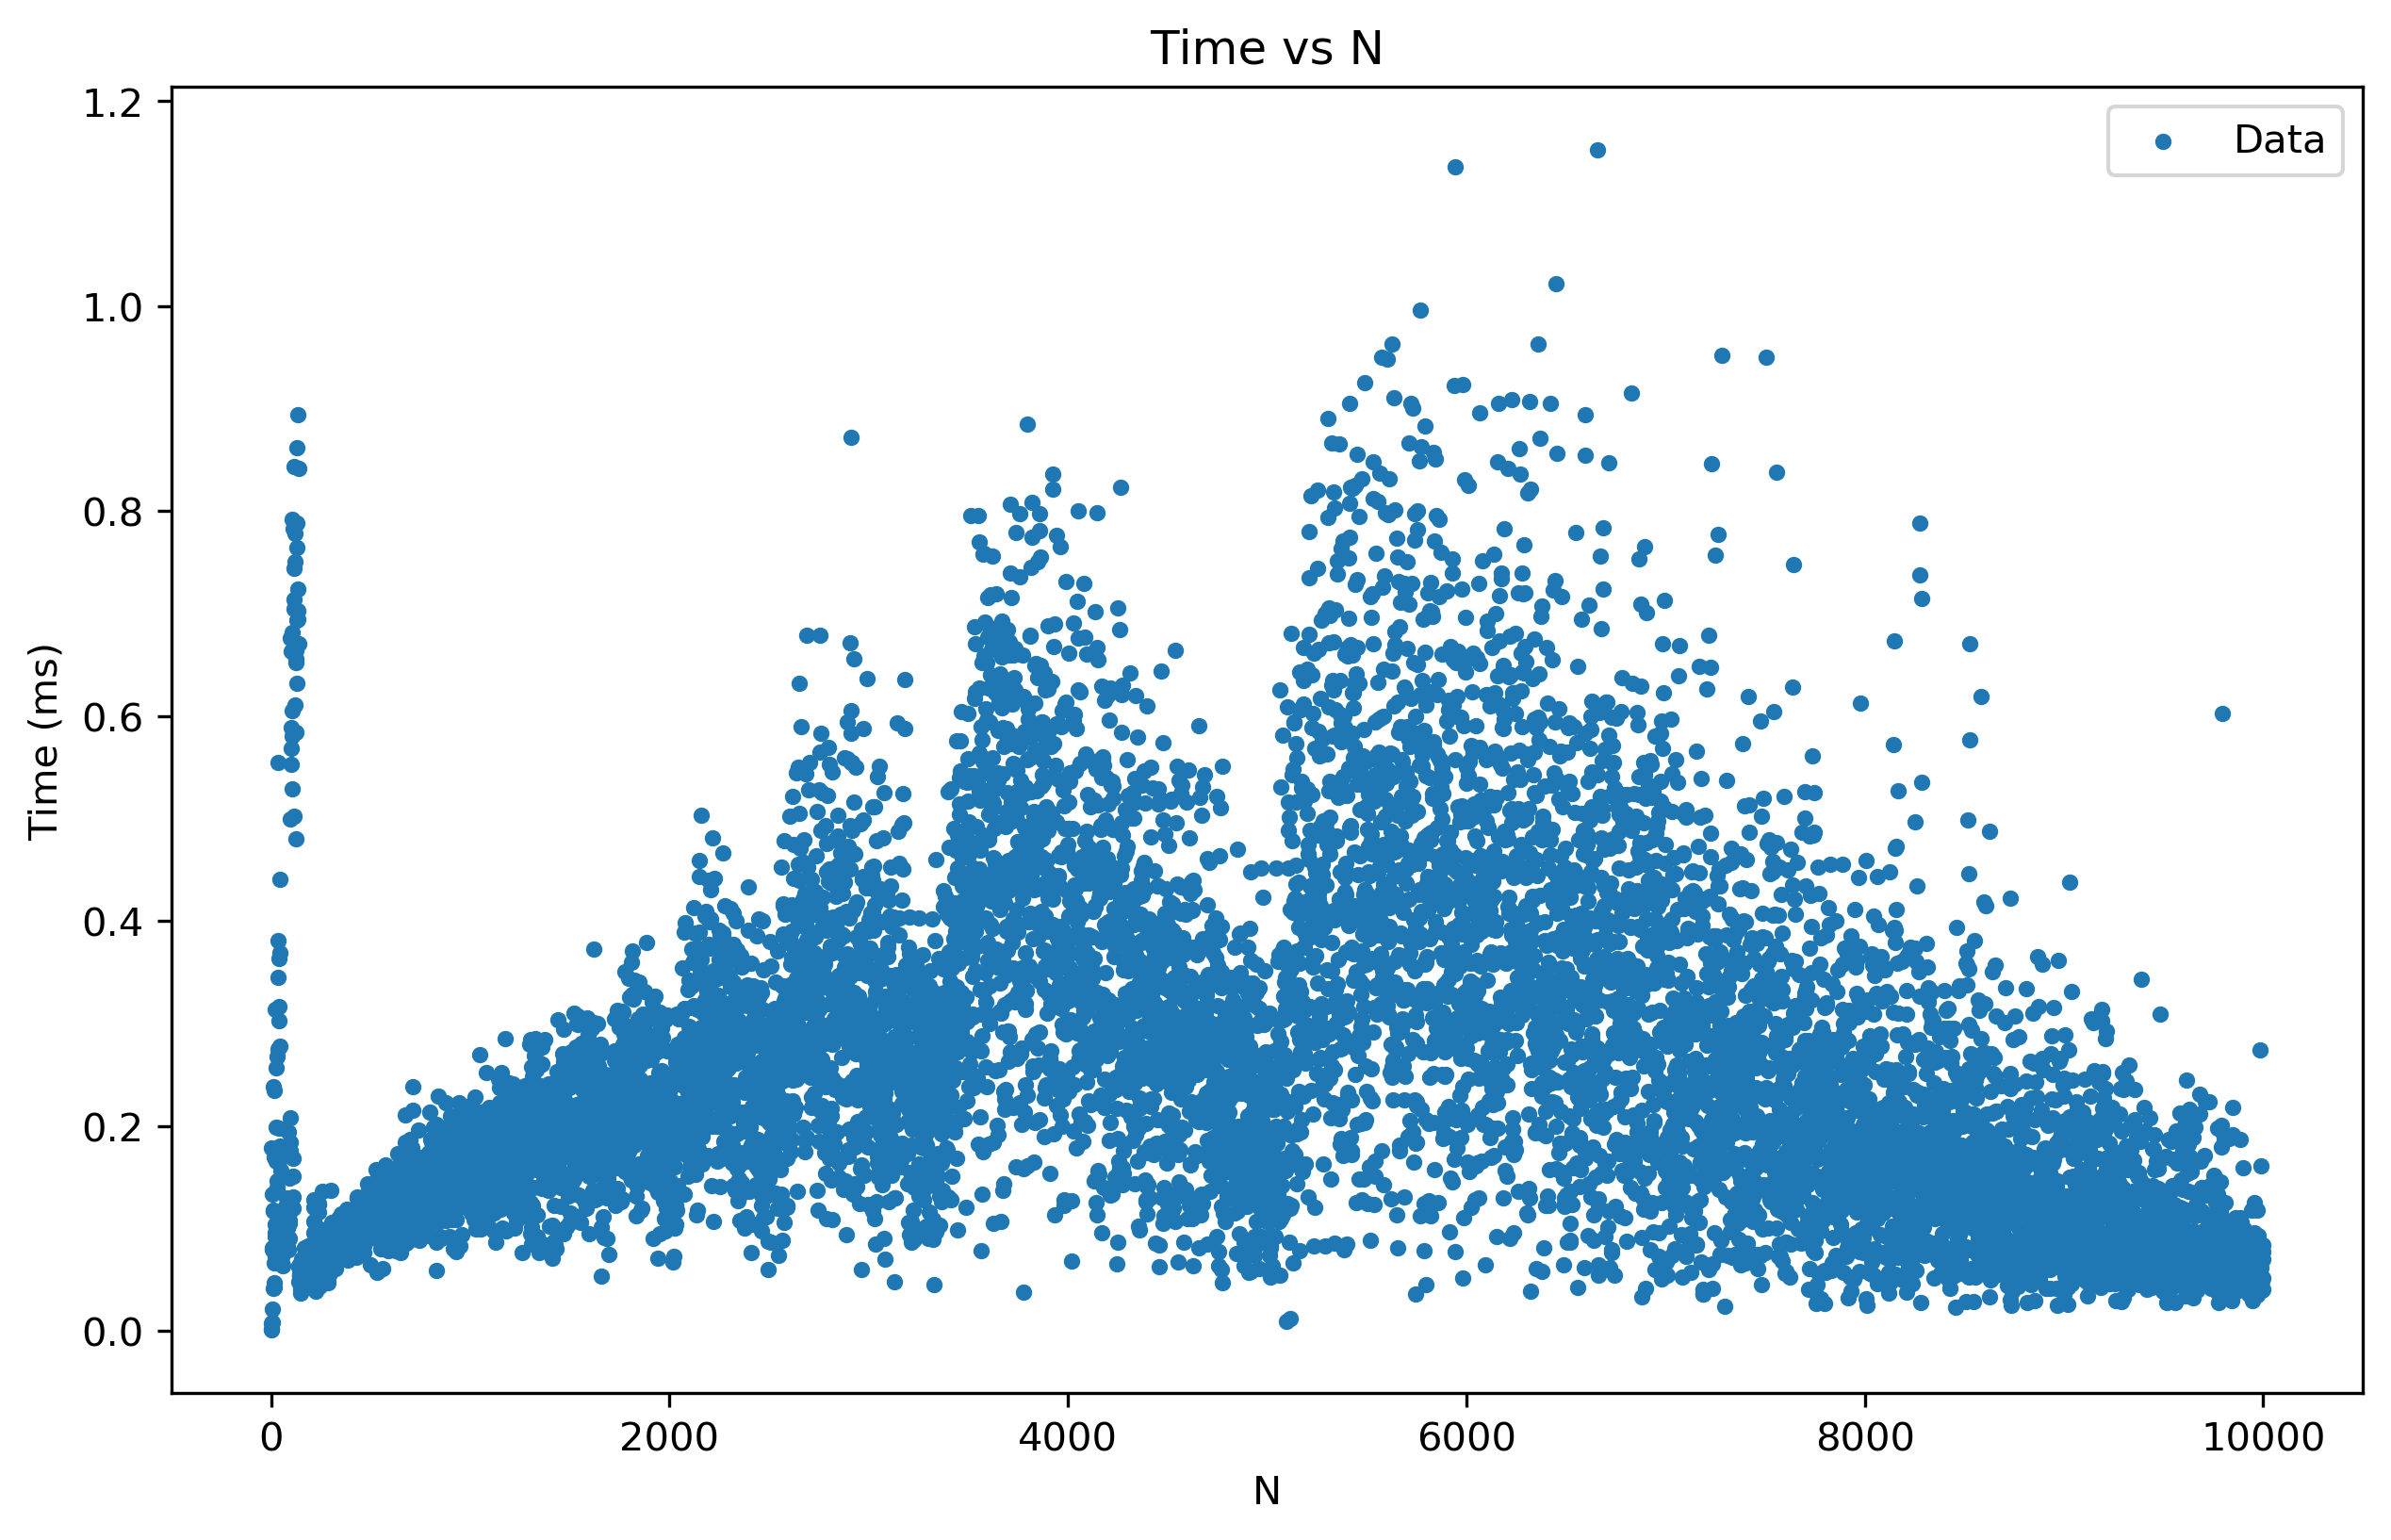
\includegraphics[width=0.7\textwidth]{chart_rules.png}
\end{center}

\emph{Tiempos tomados
utilizando la función \texttt{System.nanoTime()} de Java. Los datos
fueron generados aleatoriamente con un script de C++ cumpliendo todas
las precondiciones definidas.}

\hypertarget{anexo-2}{%
\subsubsection{4.2. Anexo 2}\label{anexo-2}}

\begin{center}
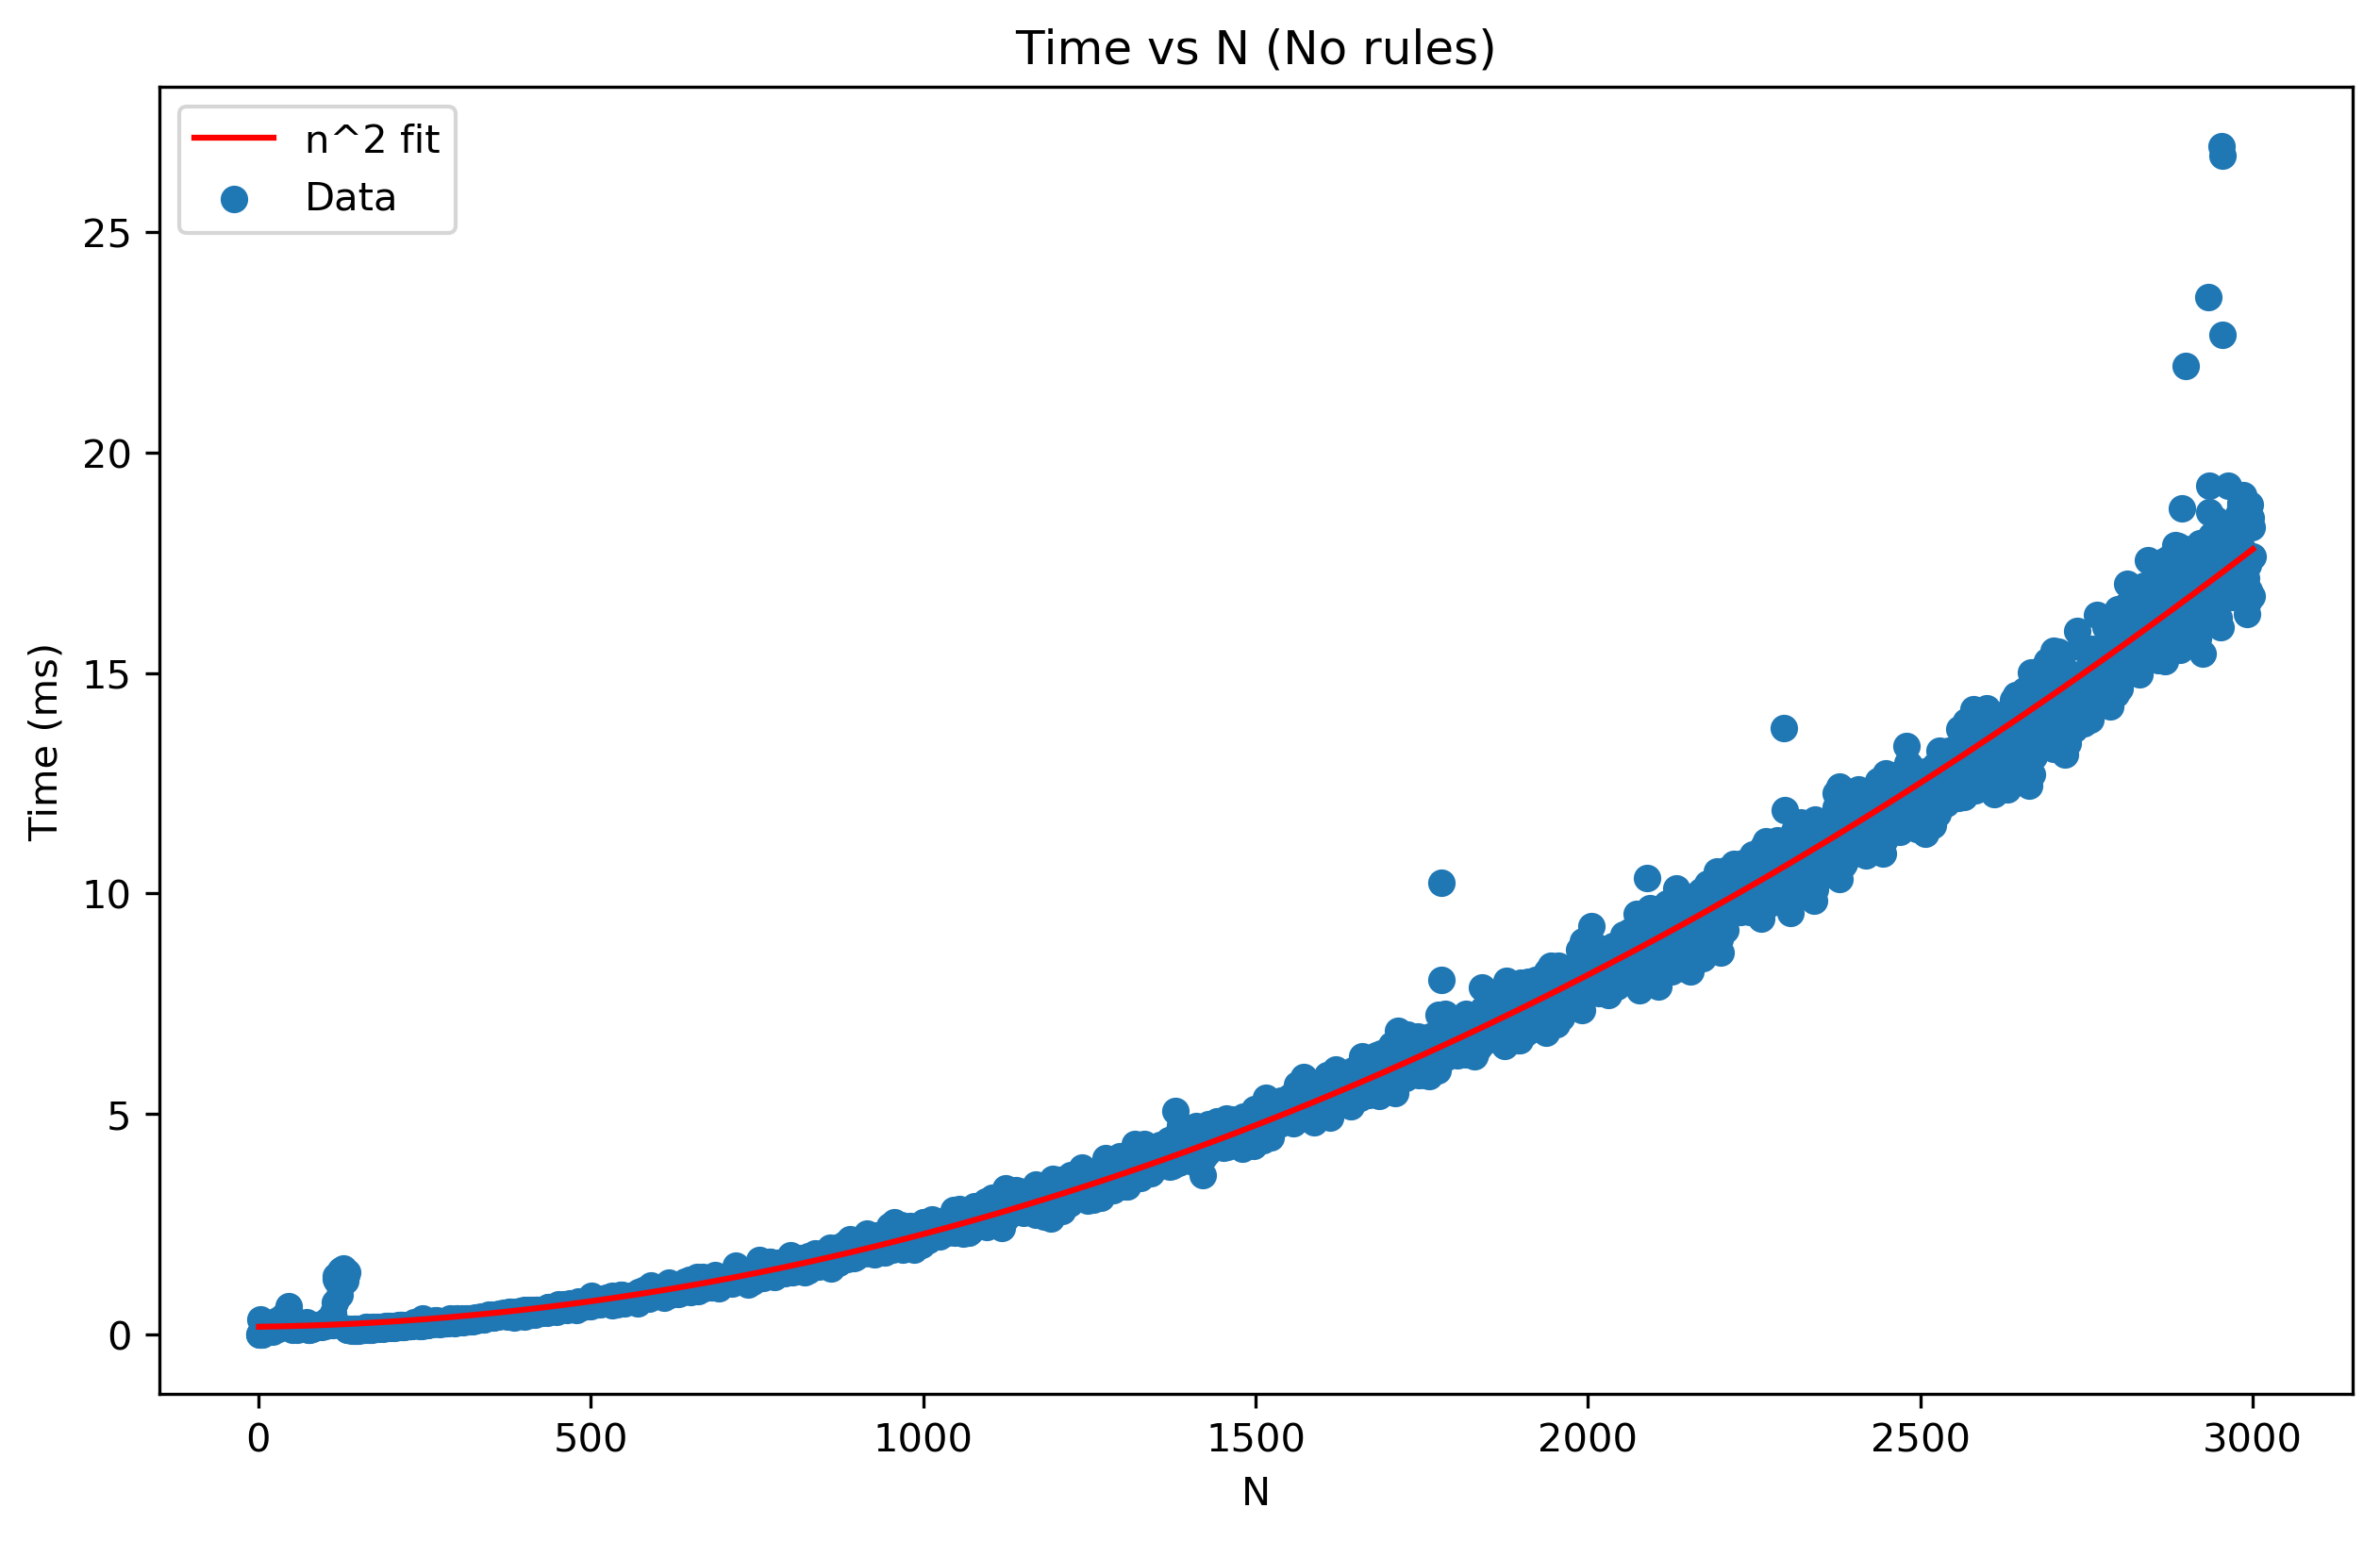
\includegraphics[width=0.7\textwidth]{chart_no_rules.png}
\end{center}

\emph{Tiempos tomados
utilizando la función \texttt{System.nanoTime()} de Java. Los datos
fueron generados aleatoriamente con un script de C++.}

\hypertarget{anexo-3}{%
\subsubsection{4.3. Anexo 3}\label{anexo-3}}

\begin{center}
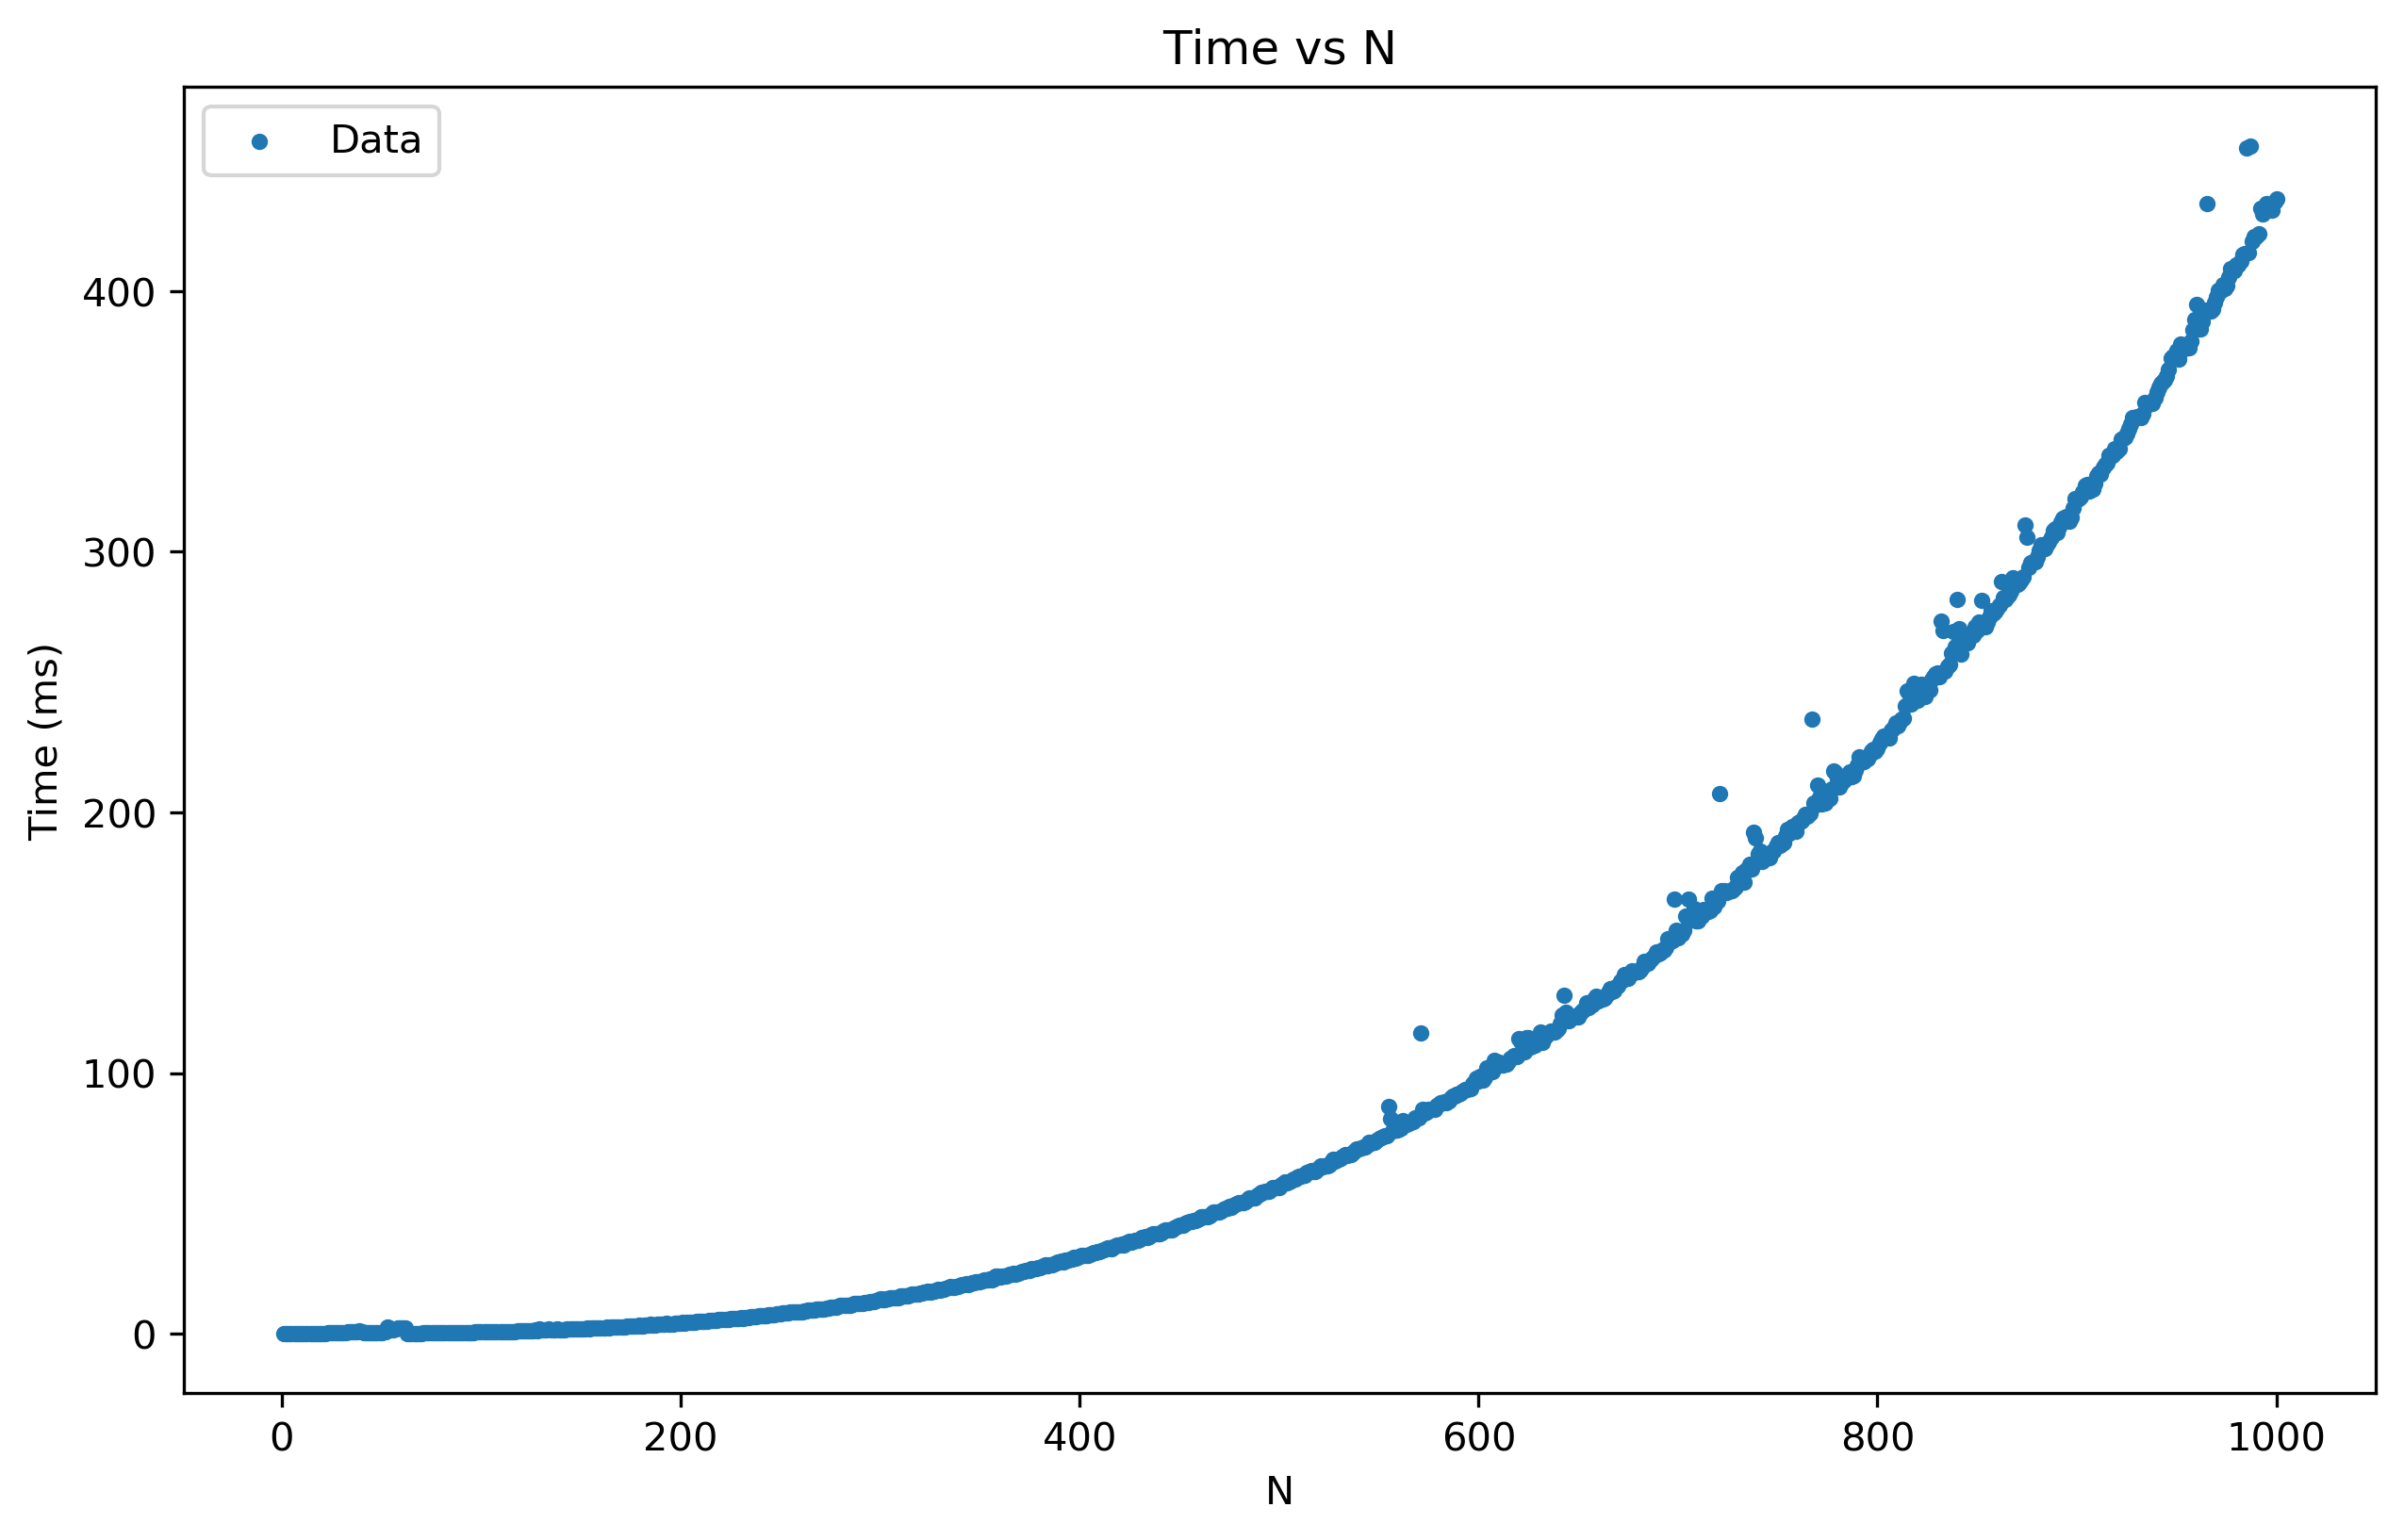
\includegraphics{chart.png}
\end{center}

\emph{Tiempos tomados utilizando la
función \texttt{System.nanoTime()} de Java. Los datos fueron generados
aleatoriamente con un script de C++.}

\end{document}
